
\subsection{Can Financing Decisions Create Value?}
\begin{frame}{\subsecname}
	\begin{itemize}
		\item Previous lectures focused on \textbf{investment decisions} (NPV criterion).
		\item This lecture shifts to \textbf{financing decisions}:
		\begin{itemize}
			\item Debt-equity mix optimization
			\item Timing of security issuance
			\item Dividend policy formulation
		\end{itemize}
		\item \textbf{Why financing matters}:
		\begin{itemize}
			\item Good financing decisions: Act as \textit{financial shock absorbers} (e.g., prevent bankruptcy)
			\item Poor financing decisions: Can trigger \textit{financial distress spiral} (e.g., Lehman Brothers)
		\end{itemize}
	\end{itemize}
	\vfill
	\footnotesize\textit{Key Insight: While investments drive growth, financing decisions determine survival.}
\end{frame}

\begin{frame}{Three Avenues for Value Creation}
	\centering
	\begin{tikzpicture}[node distance=0.5cm]
		\node (strat1) [rounded corners,fill=blue!15,text width=3.5cm,align=center] {\textbf{Market Timing} \\ {\footnotesize\textit{(e.g., IPO windows)}} \\ \tiny\textcite{baker2002market}  \\ {\tiny $\Delta \text{CAR} = +3\%$}};
		\node (strat2) [right=of strat1,rounded corners,fill=green!15,text width=3.5cm,align=center] {\textbf{Tax Arbitrage} \\ {\footnotesize\textit{(e.g., debt shields)}} \\ \tiny\textcite{graham2001payout} \\ {\tiny $\text{NPV} = 7-15\%$}};
		\node (strat3) [right=of strat2,rounded corners,fill=red!15,text width=3.5cm,align=center] {\textbf{Green Innovation} \\ {\footnotesize\textit{(e.g., green bonds)}} \\ \tiny\textcite{flammer2021corporate} \\ {\tiny $\text{CAR} = +1.3\%$}};
	\end{tikzpicture}
	\vspace{0.5cm}
	\begin{itemize}
		\item \textcolor{blue}{Short-Term}: 1–3 years (volatility-driven)
		\item \textcolor{green}{Medium-Term}: 5–10 years (structural)
		\item \textcolor{red}{Long-Term}: 10+ years (innovation-driven)
	\end{itemize}
\end{frame}

\begin{frame}{Creating Value through Market Timing: Can Firms Fool Investors?}
	\begin{itemize}
		\item Theory: Firms might create value by \textit{fooling investors} through financing tactics.
		\item Reality: Sustained deception is difficult in reasonably efficient markets.
		\begin{itemize}
			\item Over time, asset prices converge to intrinsic values.
		\end{itemize}
		\item Risks of attempting to fool investors:
		\begin{itemize}
			\item Legal sanctions
			\item Reputation loss
			\item Market corrections that reverse any gains
		\end{itemize}
		\item Common examples:
		\begin{itemize}
			\item Earnings management and aggressive accounting
			\item Insider trading
			\item Market price manipulation
		\end{itemize}
	\end{itemize}
\end{frame}

\begin{frame}{Why Market Timing Fails: The Enron Case }
	\begin{columns}
		\column{0.6\textwidth}
		\textbf{Mechanics of Collapse\parencite{healy2003fall}}:
		\begin{itemize}
			\item Hidden debt via SPEs: \$1.2B off-balance-sheet
			\item Stock price drop: \$90.75 (2000) → \$0.26 (2001)
		\end{itemize}
		\column{0.4\textwidth}
		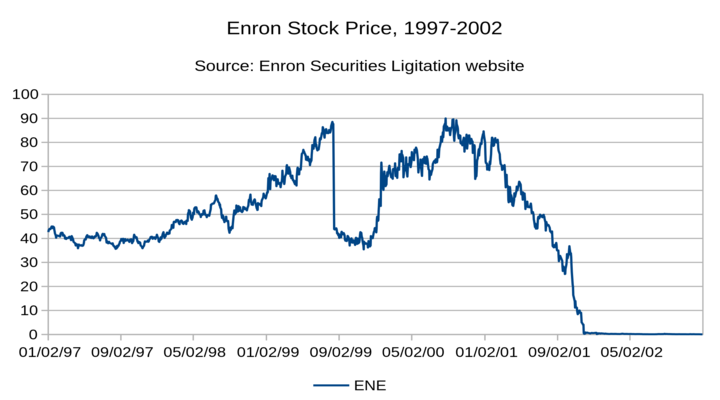
\includegraphics[width=\textwidth]{images/section1/enron_stock_chart.png}
	\end{columns}
	\vspace{0.3cm}
	\begin{alertblock}{Modern Enforcement \parencite{palantir2023}}
		AI tools (e.g., Palantir) detect anomalies in real-time. \\
		{\footnotesize\textcolor{gray}{Source: SEC 2023 Enforcement Report}}
	\end{alertblock}
\end{frame}

\begin{frame}{Reducing Costs or Increasing Subsidies: A Financing Channel}
	Certain financing structures offer explicit or implicit subsidies.
	\begin{block}{Illustration: Subsidized Bond Issuance}
		Ant Sports Co. applies for a tax-exempt, 5-year, \textyen 2 million industrial bond in Fujian to avoid relocating production to Vietnam.
		\begin{itemize}
			\item Regular debt cost: 10\%
			\item Industrial bond coupon: 5\%
			\item Annual interest savings: \textyen 100,000
		\end{itemize}
		\textbf{Question}: What is the NPV of accepting the subsidy?
	\end{block}
\end{frame}

\begin{frame}{Valuation of Subsidized Financing}
	\textbf{NPV Calculation}:
	\begin{align*}
		NPV &= \text{\textyen} 2,000,000 - \sum_{t=1}^5 \frac{\text{\textyen} 100,000}{1.1^t} - \frac{\text{\textyen} 2,000,000}{1.1^5} \\
		&= \text{\textyen} 2,000,000 - \text{\textyen} 1,620,921 \\
		&= \text{\textyen} 379,079
	\end{align*}
	\textbf{Conclusion}:  
	Ant Sports captures a \textbf{subsidy} worth \textyen 379,079 by issuing the industrial bond.

 \textbf{Interpretation}: The Fujian government provides an implicit subsidy equal to NPV via below-market rates
\end{frame}

\begin{frame}{Creating Value through Financial Innovation}
	\begin{block}{Core Idea}
		\textbf{Firms can create value by issuing new types of securities} that satisfy previously unmet investor preferences or risk-return demands.
	\end{block}
	
	\vspace{0.3cm}
	
	\begin{exampleblock}{Example: Convertible Bonds}
		\begin{itemize}
			\item \textbf{Downside protection}: Bond features limit investor losses.
			\item \textbf{Upside participation}: Embedded call option captures stock price appreciation.
			\item \textbf{Issuer benefits}: Lower financing costs and deferred equity dilution.
		\end{itemize}
	\end{exampleblock}
	
	\vspace{0.3cm}
	\begin{alertblock}{Important Caveat}
		The initial advantage often erodes quickly as competitors imitate the innovation, eliminating excess returns.
	\end{alertblock}
\end{frame}


\begin{frame}{Synthesis: Value Creation Pathways}
\begin{table}[h]
    \centering
    \resizebox{\textwidth}{!}{
	\begin{tabular}{lccp{6cm}}
		\toprule
		\textbf{Strategy} & \textbf{Persistence} & \textbf{Value Impact} & \textbf{Critical Considerations} \\
		\midrule
		Market Timing & Short-term & Low & Relies on transient mispricing; exposes firms to regulatory and reputational risks. \\
		Tax Optimization & Long-term & Medium & Requires durable alignment with legal structures and economic substance. \\
		Security Design & Medium-term & High & Demands continual adaptation to evolving investor needs and competitive imitation. \\
		\bottomrule
	\end{tabular}
    }
\end{table}

\begin{block}{Key Insights}
\begin{itemize}
	\item \textcolor{blue}{\textbf{Sustainable value}} arises from \textit{structural advantages}, not opportunistic tactics.
	\item \textcolor{green}{\textbf{Strategic imperative}}: Integrate financial engineering with superior operational execution.
\end{itemize}
\end{block}
\end{frame}
